%TEX program = xelatex
\documentclass[letterpaper,10pt]{article}
\usepackage{amsmath}
\usepackage{hyperref}
\usepackage[margin=2cm]{geometry}
\usepackage{graphicx}

\begin{document}
\title{Performance of ESPO-R5 v1.0}
\author{Pascal Bourgault, Travis Logan, Trevor J. Smith, Juliette Lavoie}
\maketitle

The assessment of the bias-adjustment performance of ESPO-R5 was inspired by the VALUE project(\cite{Maraun2015}), a framework for evaluating different bias-adjustment and downscaling methods, like the DQM method used here (see \emph{adjustment.pdf}). The framework defined a large collection of "indices" to study different aspects of the data, which can be compared to each other with "measures". Through an implementation of a subset of these indices and measures into xclim (which calls the indices "properties"), we looked at the changes brought by the bias-adjustment for many different aspects of the data. Following the VALUE project, we define 4 different aspects : marginal, temporal, multivariate and spatial. Table~\ref{tab:props} lists all properties studied for this analysis.

\begin{table}[!ht]
    \centering
    \caption{Properties used in the performance assessment of ESPO-R5v1.0}
    \begin{tabular}{l|c|c|c|l}
    \hline
    Property                               & Short name & Variables          & Aspect   & Source \\ \hline
    Mean                                   & mean       & tasmin, tasmax, pr & marginal & VALUE \\ \hline
    First percentile                       & q01        & tasmin, tasmax     & marginal & VALUE \\ \hline
    95th percentile                        & q95        & pr                 & marginal & VALUE \\ \hline
    99th percentile                        & q99        & tasmin, tasmax, pr & marginal & VALUE \\ \hline
    Dry spell frequency                    & dry\_spell\_freq & pr           & marginal & VALUE \\ \hline
    Amplitude of the annual cycle          & aca        & tasmin, tasmax     & temporal & VALUE \\ \hline
    Relative amplitude of the annual cycle & aca        & pr                 & temporal & VALUE \\ \hline
    Lag-1 autocorrelation                  & lag1       & tasmax             & temporal & VALUE \\ \hline
    Intervariable correlation (spearman)   & corr       & tasmin-tasmax, pr-tasmax & multivariate & VALUE \\ \hline
    Spatial correlograms                   & correlogram & tasmin, tasmax, pr & spatial & \cite{Francois2020} \\\hline
    First EOF                              & first\_eof & tasmin, tasmax, pr & spatial & \cite{Vrac2018} \\ \hline
    \end{tabular}
    \label{tab:props}

\end{table}

The \emph{properties} were computed on the calibration period (1981-2010) on the raw simulations, on the bias-adjusted scenarios and on the reference. The results for the raw simulations were compared to those for the reference using a \emph{measure} appropriate for that each property.\footnote{All properties in \ref{tab:props} are compared using a simple bias measure ($P_{sim} - P_{ref}$) except for the \emph{relative amplitude of the annual cycle}, which uses the ratio measure ($P_{sim} / P_{ref}$)}. This way, for each member of the ensemble, one can visualize a given property and compare the measures to assess the improvement brought by the bias adjustment. Because of performance issues, the properties and measures were not computed on the full domain of ESPO-R, but rather on three smaller regions chosen to cover different climate types.

To complement this useful but quite exhaustive collection of maps, the proportion of improved gridpoints (we'll call this indicator IMP) was found for each property. A gridpoint is said to have been improved if the bias (ratio) between the scenario and the reference is smaller (closer to 1) than the one between the raw simulation and the reference. By taking the mean accross all members of the ensemble, this allowed to have an idea of which properties were improved by the bias adjustment (those with IMP close to 100 \%), which were not impacted (IMP around 50\%) and which were worsened (IMP smaller than 50 \%). Fortunately, We do not have any properties of the latter case in this study.

As always when asserting the quality of a bias-adjustment, one must not forget that terms like "improvement" or "performance" refer to the change in comparison with the reference which is taken as the Truth in this context. Thus, the validity of bias-adjusted is limited by that reference's validity. A succint analysis of ERA5-land was done in the README at the root of this repository and it is there explained why we chose to use it as a reference, even though it has issues when compared against the observations of the AHCCD dataset (here again taken as a Truth in that context).

This whole analysis not only serves as an assessment of the performance of ESPO-R5v1.0, but also as a benchmark for the next iterations of the ESPO datasets. Here, we aim to test our performance evaluation tools and tune the list of properties to evaluate.

\section{Marginal aspects}
Detrended Quantile Mapping will adjust most properties marked as "marginal" by construction. Our algorithm divides the distribution of values for each day of the year into 50 bins and thus the percentile properties should look almost perfectly adjusted. Indeed, all members show over 90\% of improved grid points for the percentiles properties of pr and tasmax. Usually, the non-improved grid points are those where the simulation was already comparing well with the reference and indicate that there is noise (variability) in the scenario, more than anything else. This can also be seen when comparing results for members where the initial resolution was 0.44° with those for the 0.22° sources: the former systematically have stronger IMP scores than the latter. However, we can't really conclude anything else than that bilinear regridding is a worst downscaling technique than a region climate model.

Scores are lower for tasmin. Recall that here tasmin is not directly adjusted, but is rather computed from the adjusted tasmax and dtr, the daily temperature range. This indirect adjustment seems to be visible when inspecting the properties and measures, as will be shown again further down. Conclusions are very similar for the "mean" properties.

The dry spell frequency has a similar behaviour where only members with large initial biases show strong IMP. This property is also somewhat adjusted by construction during the pre-processing of precipitation data, at least for members with too many dry days, when compared to the reference. The process explained in the "Adjustment" document is mostly meant to ensure valid quantile mappings, but it does have a small effect on the final scenarios. There are still some members where the frequency of dry days is up to around 6\% greater in the scenarios then in the reference, especially over lakes. The bias is also quite consistently positive for all members and regions.

\section{Temporal aspects}
As the bias adjustment acts separately on each day of the year and, as we've seen, the scenario distribution matches well the reference one, it would be expected that the annual cycle amplitude is well adjusted. And indeed, for both temperatures, the improvement is major for all members, most showing IMP values over 90 \%. Scores are slightly weaker for precipitation, but it is here important to note than in some regions precipitation doesn't have an annual cycle as strong and and consistent as temperature. And still, IMP values are over 75 \% for two-thids of the members. Again, there a strong correlation between the improvement amount and the initial bias. Some members had really bad annual cycle amplitude patterns before the adjustment, which makes their high IMP scores almost trivial. So much so that it becomes less a measure of the performance of the bias adjustment than a measure of the bias between the simulation and the reference, see figure~\ref{fig:acapr} for example. An additionnal way to see this 

\begin{figure}
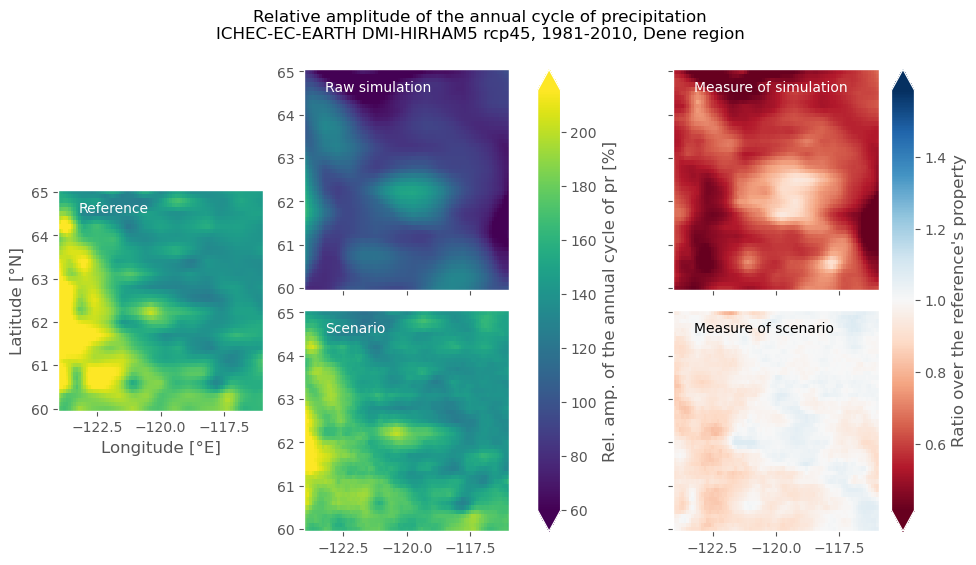
\includegraphics[width=\textwidth]{../images/aca_pr_diags.png}
\caption{Example of diagnostic maps showing a large bias betwen the simulation and the reference as well as a large improvements in the scenario.}\label{fig:acapr}
\end{figure}


Unsurprisingly, the lag-1 autocorrelation property doesn't seem to be significantly improved by the bias-adjustment. Generally, the lag-1 autocorrelation structure from the simulations is almost identical in the scenarios. Indeed, the algorithm does not adjust this aspect explicitly, but it may be interesting for futher versions of the ESPO datasets to address this issue.

\section{Multivariate aspects}
Our algorithm is inherently univariate, but the special treatment of tasmin does seem to have a strong effect on the correlation between tasmax and this variable. Most simulations of the ESPO-R5 ensemble tend to underestimate the correlation between the two variables and this bias is drastically reduced in the scenarios. If our analysis is correct, the reconstruction of tasmin from dtr and tasmax does improve that aspect of the data, while it reduced the improvement of other properties, as discussed above.

When looking at the biases in the tasmax-pr correlation, we do see large IMP values in some regions and members. In most of these cases, the initial bias between the simulations and the reference was quite large (much larger than in the tasmax-tasmin case), which leaves much room for improvement. This is visible as a strong correlation between the improvement of the measure in the scenario and it's value in the simulation.

\section{Spatial aspects}
In the lack of real benchmark values, the spatial correlograms seems to visually show an already good fit between the simulations and the reference. However, we see no improvement in the scenarios. In general, the correlogram are very similar between the simulations and the scenarios and we see no significant change in the spatial correlation length (distance where the correlation drops below a certain threshold, taken here as 0.35 for all variables). Even though we explicitly take care of adjusting the dry days frequency, we do not see the spatial correlation improvement described by \cite{Francois2020}.

\begin{thebibliography}{6}
\bibitem{Francois2020} François, B., Vrac, M., Cannon, A. J., Robin, Y., \& Allard, D. (2020). Multivariate bias corrections of climate simulations: Which benefits for which losses? Earth System Dynamics, 11(2), 537–562. https://doi.org/10.5194/esd-11-537-2020

\bibitem{Maraun2015} Maraun, D., Widmann, M., Gutiérrez, J. M., Kotlarski, S., Chandler, R. E., Hertig, E., Wibig, J., Huth, R., \& Wilcke, R. A. I. (2015). VALUE: A framework to validate downscaling approaches for climate change studies. Earth’s Future, 3(1), 1–14. https://doi.org/10.1002/2014EF000259

\bibitem{Vrac2018} Vrac, M. (2018). Multivariate bias adjustment of high-dimensional climate simulations: The Rank Resampling for Distributions and Dependences (R2D2) bias correction. Hydrology and Earth System Sciences. https://doi.org/10.5194/HESS-22-3175-2018


\end{thebibliography}
\end{document}